%%%%%%%%%%%%%%%%%%%%%%%%%%%%%%%%%%%%%%%%%
% Beamer Presentation
% LaTeX Template
% Version 1.0 (10/11/12)
%
% This template has been downloaded from:
% http://www.LaTeXTemplates.com
%
% License:
% CC BY-NC-SA 3.0 (http://creativecommons.org/licenses/by-nc-sa/3.0/)
%
%%%%%%%%%%%%%%%%%%%%%%%%%%%%%%%%%%%%%%%%%

%----------------------------------------------------------------------------------------
%	PACKAGES AND THEMES
%----------------------------------------------------------------------------------------

\documentclass{beamer}

\mode<presentation> {

% The Beamer class comes with a number of default slide themes
% which change the colors and layouts of slides. Below this is a list
% of all the themes, uncomment each in turn to see what they look like.

%\usetheme{default}
%\usetheme{AnnArbor}
%\usetheme{Antibes}
%\usetheme{Bergen}
%%%%%%%%%%\usetheme{Berkeley}
%\usetheme{Berlin}
%\usetheme{Boadilla}
%\usetheme{CambridgeUS}
%%%%%%%%%%%%\usetheme{Copenhagen}
%\usetheme{Darmstadt}
%%%%%%%%%%%%%\usetheme{Dresden}
%%%%%%%%%%%%%%%%%%\usetheme{Frankfurt}
\usetheme{Goettingen}
%\usetheme{Hannover}
%\usetheme{Ilmenau}
%\usetheme{JuanLesPins}
%\usetheme{Luebeck}
%\usetheme{Madrid}
%\usetheme{Malmoe}
%\usetheme{Marburg}
%\usetheme{Montpellier}
%\usetheme{PaloAlto}
%\usetheme{Pittsburgh}
%\usetheme{Rochester}
%\usetheme{Singapore}
%\usetheme{Szeged}
%%%%%%%%%%\usetheme{Warsaw}

% As well as themes, the Beamer class has a number of color themes
% for any slide theme. Uncomment each of these in turn to see how it
% changes the colors of your current slide theme.

%\usecolortheme{albatross}
%\usecolortheme{beaver}
%\usecolortheme{beetle}
%\usecolortheme{crane}
%\usecolortheme{dolphin}
%\usecolortheme{dove}
%\usecolortheme{fly}
%\usecolortheme{lily}
%\usecolortheme{orchid}
%\usecolortheme{rose}
%\usecolortheme{seagull}
%\usecolortheme{seahorse}
%\usecolortheme{whale}
%\usecolortheme{wolverine}

%\setbeamertemplate{footline} % To remove the footer line in all slides uncomment this line
%\setbeamertemplate{footline}[page number] % To replace the footer line in all slides with a simple slide count uncomment this line

%\setbeamertemplate{navigation symbols}{} % To remove the navigation symbols from the bottom of all slides uncomment this line
}

\usepackage{graphicx} % Allows including images
\usepackage{booktabs} % Allows the use of \toprule, \midrule and \bottomrule in tables

%----------------------------------------------------------------------------------------
%	TITLE PAGE
%----------------------------------------------------------------------------------------

\title[Detection of trading strategies]{Determinaci\'{o}n de la factibilidad de la detecci\'{o}n de estrategias de operaci\'{o}n en el mercado de divisas colombiano utilizando la informaci\'{o}n del libro de \'{o}rdenes.} % The short title appears at the bottom of every slide, the full title is only on the title page

\author{Andrea Cruz} % Your name
\institute[UN] % Your institution as it will appear on the bottom of every slide, may be shorthand to save space
{
Universidad Nacional de Colombia\\ % Your institution for the title page
\medskip
\textit{amcruzm@unal.edu.co}\\ % Your email address\\
\medskip
\medskip
Advisor: German Hernandez\\
Universidad Nacional de Colombia\\ 
\textit{gjhernandezl@unal.edu.co}
}
\date{\today} % Date, can be changed to a custom date

\begin{document}

\begin{frame}
\titlepage % Print the title page as the first slide
\end{frame}

\begin{frame}
\centering
\textbf{\color[rgb]{0,0,1} \LARGE Determining feasibility of trading strategies detection using Order Book Information from the Colombian currency market}
% The short title appears at the bottom of every slide, the full title is only on the title page

\end{frame}

\begin{frame}
\frametitle{Overview} % Table of contents slide, comment this block out to remove it
\tableofcontents % Throughout your presentation, if you choose to use \section{} and \subsection{} commands, these will automatically be printed on this slide as an overview of your presentation
\end{frame}

%----------------------------------------------------------------------------------------
%	PRESENTATION SLIDES
%----------------------------------------------------------------------------------------
\section{Introduction}

\subsection{Financial Markets}
\begin{frame}
\frametitle{Financial Markets}

\begin{figure}
	\centering
		\includegraphics[scale=0.5]{GeneralMarketDescription.png}
	\caption{Market need vs. Available information (Candlestick figure taken from \href{http://stackoverflow.com/questions/12173306/jfreechart-timeseries-and-candlestick-on-the-same-chart}a).}
	\label{fig:GeneralMarketDescription}
\end{figure}
\end{frame}

\subsection{Timescale Aggregations}
\begin{frame}
\frametitle{Timescale Aggregations}
\begin{figure}
    \centering
		\begin{tabular}{c c}
        \includegraphics[width=0.3\textwidth,height=0.3\textwidth]{AppleMonatJun2016.png} &
        \includegraphics[width=0.3\textwidth,height=0.3\textwidth]{Apple5TageJun2016.png} \\
    \scriptsize (a) Candlesticks for one month. & \scriptsize (b) Candlesticks for five days.\\		
        \includegraphics[width=0.3\textwidth,height=0.3\textwidth]{Apple1TagJun2016.png} &
        \includegraphics[width=0.3\textwidth,height=0.3\textwidth]{Apple1TagAnnährung.png} \\
    \scriptsize (c) Candlesticks for one day. & \scriptsize (d) Candlesticks for one hour. \\
		\end{tabular}	
    \caption{Apple Inc. Candlesticks charts retrieved from Yahoo Finance (July 13th, 2016).}\label{fig:TrendHA}
\end{figure}
\end{frame}


\subsection{Alternative Prediction Sources}
\begin{frame}
\frametitle{Alternative Prediction Sources}
\begin{figure}
    \centering
		\begin{tabular}{c c}
        \includegraphics[width=0.4\textwidth,height=0.3\textwidth]{world-trends.jpg} &
        \includegraphics[width=0.4\textwidth,height=0.3\textwidth]{NachrichtenGoogle.png} \\
    \scriptsize (a) World trends. & \scriptsize (b) News (Retrieved from google.de).\\		
        \includegraphics[width=0.4\textwidth,height=0.3\textwidth]{fundamental-analysis.jpg} &
        \includegraphics[width=0.4\textwidth,height=0.3\textwidth]{SozialeNetwerke.png} \\
    \scriptsize (c) Fundamental Analysis. & \scriptsize (d) Social Networks. \\
		\end{tabular}	
    \caption{Other kind of prediction sources.}\label{fig:TrendHA}
\end{figure}

\end{frame}

\subsection{Limit Order book}

\begin{frame}
\frametitle{Limit Order book Information}

Hypothesis: the use LOB dynamics information will produce more effective trading strategies.

\begin{figure}
	\centering
		\includegraphics[scale=0.45]{MenschenBuchRechnerBild.png}
	\caption{Broker's exclusive source of information.Images taken from \cite{cruz}}
	\label{fig:Introduction1}
\end{figure}
\end{frame}


\begin{frame}
\frametitle{Limit Order book Dynamics}

A more powerful tool:

\begin{figure}
	\centering
		\includegraphics[scale=0.45]{OrderBook.png}
		\caption{Order Book Dynamics. Images taken from \cite{cruz}}
	\label{fig:Introduction1}
\end{figure}


\end{frame}

\subsection{Forex Markets}
\begin{frame}
\frametitle{Forex Markets}

\begin{figure}
	\centering
		\includegraphics[scale=0.6]{FinancialMarkets.png}
	\caption{FX markets experienced a growth rate of 32.5 \% in the last three years, with the United
States Dollar as the most traded currency[50]. This information presents the USD behavior
analysis as a still interesting research area.}
	\label{fig:FinancialMarkets}
\end{figure}

\end{frame}

\begin{frame}
\frametitle{Colombian Bulk Forex Market}

\begin{itemize}
	\item Dollar buy and sell transactions are spot contracts, i.e. the transaction and its fulfillment are made on the same day. A trader buying dollars through SET-FX, receives and pays the product the same day. This market operates on workdays between 8:00 a.m. and 1:00 p.m.
	\item “SET ICAP FX S.A.” manages the trading platform SET-FX which is supported by the strategic alliance between its shareholders the Colombia Stock Exchange and SIF ICAP Mexico, the latter, a subsidiary of the Mexican Stock Exchange and ICAP PLC in London.
\end{itemize}

\end{frame}

%------------------------------------------------


%------------------------------------------------
\section{Thesis Goal} % Sections can be created in order to organize your presentation into discrete blocks, all sections and subsections are automatically printed in the table of contents as an overview of the talk
%------------------------------------------------

\begin{frame}
\frametitle{Main goal}

To study trading strategies using order book information from the Colombian Forex Market and its potential in the construction of predicting models.

\begin{figure}
	\centering
		\includegraphics[scale=0.4]{Goals1.png}
	\label{fig:Goals1}
\end{figure}


\end{frame}

%---------------------------------------------------------------
\section{Results}
%---------------------------------------------------------------

\subsection{Visualization}
%---------------------------------------------------------------
\begin{frame}
\frametitle{Proposed visualization}
\begin{figure}
	\centering
		\includegraphics[scale=0.3]{Visualization1.png}
	\caption{Evolution of the proposed visualization.}
	\label{fig:Visualization1}
\end{figure}
\end{frame}

\begin{frame}
\frametitle{Similar tools}
\begin{figure}
	\centering
		\includegraphics[scale=0.4]{SimilarVisualizations.png}
	\caption{Similar visualization tools \cite{BookMap15},\cite{Todd},\cite{chris13},\cite{cruz}.}
	\label{fig:Visualization1}
\end{figure}
\end{frame}

\subsection{Detection of trading strategies}
%---------------------------------------------------------------

\begin{frame}
\frametitle{Dataset description}
\begin{itemize}
	\item Experiments were conducted using real tick data of foreign exchange rate USDCOP from March to May of 2012.
	\item LOB provides information about time, price and volume for every request in the market; this information was summarized every minute, in a price range of 120 COP in the best quotes, using a 20 cents mark up. 
	\item Volumes were quantized in levels of USD 250,000, which is the minimum trading volume for this market. The maximum volume observed for a particular order during the analyzed period was 43.5 USD millions. The maximum price observed was 1,862.6 COP and the minimum was 1,742.2 COP. 
\end{itemize}
 
\end{frame}

\begin{frame}
\frametitle{Heatmap based approach}

\begin{figure}
	\centering
		\includegraphics[scale=0.3]{Methodology1.png}
	\label{fig:Methodology1}
\end{figure}

\end{frame}

\begin{frame}
\frametitle{Wavelets}

\begin{figure}
\centering
\begin{subfigure}
  \centering
  		\includegraphics[scale=0.5]{curiositoV1.png}
	\label{fig:curiositoV1}
\end{subfigure}%
\begin{subfigure}
  \centering
\includegraphics[scale=0.5]{curiositoV2.png}
	\label{fig:curiositoV2}
	\end{subfigure}
	\caption{Result of the application of Haar wavelet transform over an image.}
	\label{fig:test}
	\end{figure}
\end{frame}

\begin{frame}

\begin{columns}
\column{.45\textwidth}
\begin{center}
With the aim of exploring different resolution levels, the subsets were compressed in four stages using Haar Wavelet Transform. Both sets of coefficients were employed independently. This was a preprocessing step and later the same procedure for the heatmap based approach was followed.
\end{center}
\column{.45\textwidth}
\begin{figure}
		\centering
			\includegraphics[scale=0.5]{wavelets2.png}
		\caption{Effect on the image's size of using Haar Wavelet transform.}
		\label{fig:wavelets2}
	\end{figure}
\end{columns}
\end{frame}

\begin{frame}
\frametitle{Heatmap based approach vs. Wavelets based approach}

\begin{figure}
	\centering
		\includegraphics[scale=0.3]{chart1.png}
	\label{fig:chart1}
\end{figure}
\end{frame}

\begin{frame}
\frametitle{Heatmap based approach vs. Wavelets based approach}

\begin{figure}
	\centering
		\includegraphics[scale=0.3]{chart2.png}
	\label{fig:chart2}
\end{figure}
\end{frame}


\begin{frame}
\frametitle{Behavior within and outside a Global Trend}

\begin{itemize}
	\item \small The Heatmap and the Wavelet approach were applied over the whole dataset and the performance difference between datasets suggests the existence of seasonal patterns \cite{Jian09a}.
	\item \small To test this hypothesis, two subsets with global opposite trends were identified using moving average and the performance of 400 different pattern sizes was evaluated using only the hash function. 
	\item \small In this scenario, 35 pattern sizes achieved accuracy higher than 0.6 in the first subset, when tested in the opposite trend, only 4 kept their accuracy.
\end{itemize}

\end{frame}


\begin{frame}
\frametitle{Behavior within and outside a Global Trend}
\begin{figure}
		\centering
			\includegraphics[scale=0.3]{GlobalTrend.png}
		\caption{Patterns accuracy within and outside a global trend.}
		\label{fig:globalTrend}
	\end{figure}
\end{frame}

\begin{frame}
\frametitle{Adaptive Method}

\begin{enumerate}
	\item \small Make an initial training stage in which a general market trend is identified.
  \item \small Every time that a new sample arrives for classification, recalculate the probabilities associated to each trend for the patterns found in the sample.
  \item \small When the count for a new pattern apparitions reaches an specific amount and its probability of being associated with a determined trend surpasses a threshold, add that pattern to the informative frequent patterns' dictionary.
  \item \small When the count of misclassifications for a pattern from the informative frequent patterns' dictionary reaches an specific number or when its probability of being associated with a determined trend falls to a determined threshold, remove that pattern from the informative frequent patterns' dictionary.
\end{enumerate}
\end{frame}

\begin{frame}
\frametitle{Adaptive Method}
\small The previous procedure was tested for 300 different patterns' sizes, producing  29 configurations where patterns highly associated with a trend were found and whose accuracy was above 0.6. From those 29 configurations, 10 produce 5 or more predictions on the dataset. Three different convergence behaviors were found as it could be observed in figure \ref{fig:Adaptive}.
\end{frame}


\begin{frame}
\frametitle{Adaptive Method}

There is a need of identifying when a labeled pattern starts to lose the ability to predict the trend. For this reason we presented an online method for informative frequent patterns identification.

\begin{figure}
	\centering
		\includegraphics[scale=0.10]{Adaptive.png}
		\caption{Different convergence behaviors found for the adaptive method.}
	\label{fig:Adaptive}
\end{figure}
\end{frame}

\begin{frame}
\frametitle{Cluster approach}
\begin{columns}
\column{.5\textwidth}
\begin{itemize}
	\item Introduces the idea of similarity among patterns.
	\item Reduces the patterns' search universe to 13 clusters.
	\item This study is based on the trading data of the manual market of Colombian Forex Market from May 2nd until October 10 during the year 2014. For being more informative, the order book section closer to the spread was chosen for the exploration[45].
\end{itemize}
\column{.45\textwidth}
\begin{figure}[]
	\centering
		\includegraphics[scale=0.5]{bagOfWords.png}
	\caption{\footnotesize Bag\-of\-visual\-ngrams general scheme provided by Lopez Monroy et al. \cite{draw}}
	\label{fig:bagOfWords}
\end{figure}
\end{columns}
\end{frame}

\begin{frame}
\frametitle{Cluster approach}

\begin{itemize}
	\item Time-price-volume matrix was chopped and adjusted for working in regions near to the spread.
	\item The matrix was traversed using tiles of 30x30.
	\item Every pattern was assigned to a cluster using k-means.
	\item In a new matrix, the size of each cluster was registered in order to keep track of the frequency at which patterns were assigned to every cluster.
	\item Finally, each cluster was labeled with the observed trend when the probability of being associated to it was higher than 0.55.
\end{itemize}


\end{frame}

\begin{frame}
\frametitle{Cluster approach}
\begin{figure}
	\centering
		\includegraphics[scale=0.25]{results.png}
		\caption{Clusters and their performance.}
	\label{fig:results}
\end{figure}
\end{frame}

\begin{frame}
\frametitle{Variable Time Horizon and Sliding Window}
\begin{itemize}
	\item This method used five different window arrangements:Vertical arrangement, Horizontal arrangement, Haar Wavelet Transform arrangement, sliding window arrangement and adjacent window arrangement.
	\item  This method used six different time horizons: 2, 4, 6, 10, 16 and 30
minutes.
	\item There are two important factors to be measured: first, the potential profit generated for each method and second, the risk level associated to each method. The mean of the returns allows to win insights about each method’s potential profit. With the purpose of providing a reliability measure, the returns variance was normalized.
\end{itemize}
\end{frame}

\begin{frame}
\begin{figure}
    \centering
		\begin{tabular}{c c}
        \includegraphics[scale=0.5]{TWDReturns.png} &
        \includegraphics[scale=0.5]{TWDReliabilities.png} \\
      \scriptsize (a) Returns' means over the whole  & \scriptsize (b) Reliabilities means over the \\ 
			\scriptsize dataset. & \scriptsize whole dataset.\\
		\end{tabular}	
\caption{Returns and Reliabilities Means over the whole dataset using vertical and horizontal window arrangement}\label{fig:TrendTWD}
\end{figure}
\end{frame}

\begin{frame}
\begin{figure}
    \centering
		\begin{tabular}{c c}
		
        \includegraphics[scale=0.5]{TrendVSReturn.png} &
        \includegraphics[scale=0.5]{TrendVSReliability.png} \\
    \scriptsize (a) Returns' means over a subset  & \scriptsize (b) Reliability means over a subset\\
    \scriptsize using Vertical Sliding Window & \scriptsize using Vertical Sliding Window\\
		\scriptsize arrangement. & \scriptsize arrangement.\\
        \includegraphics[scale=0.5]{TrendVAReturn.png} &
        \includegraphics[scale=0.5]{TrendVAReliability.png} \\
    \scriptsize (c) Returns' means over a subset using & \scriptsize (d) Reliability means over a subset\\
		\scriptsize  using Vertical Adjacent Window & \scriptsize using Vertical Adjacent Window\\
		\scriptsize arrangement. & \scriptsize arrangement.\\
		\end{tabular}	
    \caption{Returns and Reliabilities means over the same subset displaying a clear trend using different Window arrangements.}\label{fig:TrendHA}
\end{figure}
\end{frame}

\begin{frame}
\begin{figure}
    \centering
		\begin{tabular}{c c}
        \includegraphics[scale=0.5]{TrendHSReturn.png} &
        \includegraphics[scale=0.5]{TrendHSReliability.png} \\
    \scriptsize (e) Returns' means over a subset & \scriptsize (f) Reliability means over a subset \\
    \scriptsize using Horizontal Sliding Window & \scriptsize using Horizontal Sliding Window\\
		\scriptsize arrangement. & \scriptsize arrangement.\\
        \includegraphics[scale=0.5]{TrendHAReturn.png} &
        \includegraphics[scale=0.5]{TrendHAReliability.png} \\
    \scriptsize (g) Returns' means over a subset & \scriptsize (h) Reliability means over a subset \\
		\scriptsize using Horizontal Adjacent Window & \scriptsize using Horizontal Adjacent Window \\
		\scriptsize arrangement. & \scriptsize arrangement.\\
		\end{tabular}	
    \caption{Returns and Reliabilities means over the same subset displaying a clear trend using different Window arrangements.}\label{fig:TrendHA}
\end{figure}
\end{frame}

\section{Conclusions}

\begin{frame}
\frametitle{Conclusions}
\begin{itemize}
	\item A systematic literature review about the Order Book was presented, there is no evidence of previous work made based on the LOB for the Colombian Forex Market until the writting date of the second chapter.
	\item  A methodology which allows representing properly the Colombian Forex Market Order Book information dynamics is presented. The visualization tools presented in this work, can provide the user with a global understanding of a selected time interval in the Colombian Forex Market.
\end{itemize}

\end{frame}

\begin{frame}
\frametitle{Conclusions}
\begin{itemize}
	\item Wavelet Heatmap visualization presents in a summarized and efficient way the order book information.
	\item A trading strategies detection system for the Colombian Forex Market using Order Book information was designed by means of a frequent patterns exploration approximation.
\end{itemize}

\end{frame}

\begin{frame}
\frametitle{Conclusions}
\begin{itemize}
	\item Given the seasonality of the found patterns, the presented strategy was reformulated as an adaptive strategy which detects when a pattern is losing predictability in order to start a new training stage for detecting new informative patterns.
	\item The performace of the proposed system in supporting the financial decision making process in the Colombian Forex Market was evaluated.
\end{itemize}

\end{frame}

%------------------------------------------------
\section{Main Contributions}
%------------------------------------------------

\begin{frame}
\frametitle{Main Contributions}
\small The following is the summary of the main contributions of this work:\\
\textbf{Forex Market Order Book Visualization}\\
A Forex Market Order Book Visualization is presented. This visualization provides the trader with a framework which allows the interpretation of large sections of the limit order book at a glance. It shows relationships between price, volume and time directly.\\
This work was published as a contributed talk named ((Order Book Microstructure Visualization: The case of Colombian High- Frequency Foreign Market. XIII Latin American Congress of Probability and Mathematical Statistics CLAPEM. September, 2014.))\\
\textbf{Efficient Trend Predicting LOB Patterns Dictionary Building}\\ 
Algorithms for Frequent Patterns Exploration are presented. These algorithms have reduced the amount of time required for mining a dataset up to two orders of magnitude depending on the pattern size, thanks to the use of a pattern summary function. The use of the Haar Transform, in some time windows, can reduce the initial dataset without loss of accuracy for the classifier, so it reduces the amount of non valuable information.
\end{frame}

\begin{frame}
\frametitle{Main Contributions}
\small\textbf{Cluster Based Patterns Identification using Bag of Words}\\
Algorithms for association between frequent patterns and a specific trend are depicted. These algorithms allow calculating the probability of each pattern of being associated with a bearish trend, a bullish trend or with no trend, labeling each pattern accordingly. The use of these algorithms allowed to detect patterns seasonality in the Colombian Forex Market Order Book.\\
This work was presented under the title ((Market Trend Visual Bag of Words Informative Patterns in Limit Order Books)) in the 6th Annual Stevens Conference on High Frequency Finance and Analytics (HF2015) that was held on October 29th-31st, 2015 at Stevens Institute of Technology, Hoboken, NJ, USA. It was published under the same title in the International Conference on Computer Science Proceedings. San Diego, California, U.S.A. (ICCS2016).
\textbf{Effective Trend Predicting LOB Patterns Dictionary}\\
Further work on this topic was submitted to the 39th edition of the German Conference on Artificial Intelligence that will be held on September 26th-30th, 2016 in Klagenfurt, Austria. The title of this contribution is ((Liquidity Patterns Identification with Variable Time Horizon Using Bag of Words)). It is currently under peer revision.\\
\end{frame}
%------------------------------------------------
\section{Future Work}
%------------------------------------------------
\begin{frame}
\frametitle{Future Work}
The fact that the proposed strategies provide useful results with a relatively small dataset from one single currency, throws as a natural consequence the need of testing them in broader datasets and new assets, even for portfolio selection. 

\begin{figure}
	\centering
		\includegraphics[scale=0.5]{futureWork.png}
	\label{fig:futureWork}
\end{figure}

\end{frame}

\begin{frame}
\frametitle{Future Work}
On the other hand, an important feature of the Wavelet based approach is that is highly parallelizable, allowing easy implementation in distributed systems such as GPUs. In order to reduce latency, it would be useful to implement the presented algorithms directly on hardware, for instance in a FPGA.

\begin{figure}
	\centering
		\includegraphics[scale=0.5]{futureWork2.png}
	\label{fig:futureWork2}
\end{figure}

\end{frame}

\section{References}

\begin{thebibliography}{X}

\bibitem{Ahmed09} [1] Ahmed, M., Chai, A., Ding, X., Jiang, Y., & Sun, Y. (2009). Statistical Arbitrage in High Frequency Trading Based on Limit Order Book Dynamics, 1-26.

\bibitem{Ahn05} [2] Ahn, H.-J., Cai, J., & Cheung, Y. L. (2005). Price clustering on the limit-order book: Evidence from the Stock Exchange of Hong Kong. Journal of Financial Markets, 8(4), 421-451.

\bibitem{Bates03} [3] Bates, R. G., Dempster, M. A. H., & Romahi, Y. S. (2003). Evolutionary reinforcement learning in FX order book and order flow analysis. In 2003 IEEE International Conference on Computational Intelligence for Financial Engineering, 2003. Proceedings. (pp. 355-362). IEEE. 

\bibitem{Bloom05} [4] Bloomfield, R., O'Hara, M., & Saar, G. (2005). The "`make or take"' decision in an electronic market: Evidence on the evolution of liquidity. Journal of Financial Economics, 75(1), 165-199.

\bibitem{BookMap15} [5] BookMap by VeloxPro. (2015, October 8). Retrieved from \url{http://www.bookmap.com/}.

\bibitem{brey03} [6] Breymann W., Dias A., Embrechts P.: Dependence structures for multivariate high-frequency data in finance. Quantitative Finance Vol. 3, Iss. 1. (2003)

\bibitem{Chen} [7] Chen, M.; Ebert, D.; Hagen, H.; Laramee, R.S.; van Liere, R.; Ma, K.-L.; Ribarsky, W.; Scheuermann, G.; Silver, D., "Data, Information, and Knowledge in Visualization," Computer Graphics and Applications, IEEE , vol.29, no.1, pp.12,19, Jan.-Feb. 2009

\bibitem{Cheng09} [8] Cheng, W., Liu, S., Jiao, H., & Qiu, W. (2009). How Does Limit Order Book Information Affect Trading Strategy and Market Quality: Simulations of an Agent-Based Stock Market. In 2009 International Conference on Management and Service Science (pp. 1-4). IEEE.

\bibitem{chris13} [9] Christensen H. L., Turner R. E., Hill S. I., Godsill S.J.: Rebuilding The Limit Order Book: Bayesian Inference on Hidden States. Quantitative Finance. pp. 1779-1799J. (2013)

\bibitem{Cont10} [10] Cont, Stoikov, and Talreja: A Stochastic Model for Order Book Dynamics. Operations Research Vol. 58, No. 3, May - June 2010, pp. 549 - 563 issn 0030 - 364X eissn 1526 - 5463  10  5803  0549 in.

\bibitem{cruz} [11] Cruz, A., Nino. J., Sandoval. J., Rincon, J., Hernandez, G.: Market Trend Visual Bag of Words Informative Patterns in Limit Order Books. International Conference on Computer Science Proceedings. San Diego, California, U.S.A. (2016)

\bibitem{dani02} [12] Danielsson J., Payne R.: Real trading patterns and prices in spot foreign exchange markets, Journal of International Money and Finance, Volume 21, Issue 2, April 2002, Pages 203-222, ISSN 0261-5606, \url{http://dx.doi.org/10.1016/S0261-5606(01)00043-2}. (2002)

\bibitem{draw} [13]Lopez-Monroy A. P., Gomez, M. M., Escalante, H. J.,  Cruz-Roa, A. and Gonzalez, F. A. Bag-of-visual-ngrams for histopathology image classification, in Proc. of SPIE 8922, 2013, p. 89220P.

\bibitem{Dono} [14] Donoho, D. and Johnstone, I. Ideal spatial adaptation via wavelet shrinkage. Biometrika, 81(3):425-455, 1994.

\bibitem{Eis07} [15] Eisler, Z., Kertesz, J., Lillo, F.: The Limit Order Book on Different Time Scales, arXiv.org, Quantitative Finance Papers 0705.4023, May 2007. [Online]. Available: \url{http://ideas.repec.org/p/arx/papers/0705.4023.html} (2007)

\bibitem{Farmer04} [16] Farmer, J. Doyne and Patelli, Paolo and Zovko, Ilija I., The Predictive Power of Zero Intelligence in Financial Markets (February 9, 2004). AFA 2004 San Diego Meetings.

\bibitem{Flet10} [17] Fletcher, T., Hussain, Z., & Shawe-Taylor, J. (2010). Multiple Kernel Learning on the Limit Order Book. In WAPA (pp. 167-174).

\bibitem{setfx} [18] Foreign Exchange Transaction Electronic System (Set-FX), \url{http://www.set-fx.com/index.html}

\bibitem{Forni01} [19] Forni, M., & Lippi, M. (2001). The generalized dynamic factor model: Representation theory. ECONOMETRIC THEORY, 17(6), 1113-1141.

\bibitem{Gabor} [20] Gabor,D. Theory of communication. J. IEE, 93:429-457, 1946.

\bibitem{Gould13} [21] Gould, M. D., Porter, M. A., Williams, S., McDonald, M., Fenn, D. J. and Howison, S. D. Limit order books.  Quantitative Finance, Vol. 13, No. 11, 1709–1742. 2013.

\bibitem{Hall07} [22] Hall, A. D., & Hautsch, N. (2007). Modelling the buy and sell intensity in a limit order book market. Journal of Financial Markets, 10(3), 249-286. 

\bibitem{Harris54} [23] Harris, Zellig S. Distributional structure. Word, Vol 10, 1954, 146-162.

\bibitem{Hsin07} [24] Hsin, P.-H., & Wang, M.-C. (2007). Information Indicators of Limit Order Book and Optimal Dynamic Order Submission Strategy. In Second International Conference on Innovative Computing, Informatio and Control (ICICIC 2007) (pp. 197-197). IEEE. 

\bibitem{Huang12} [25] Huang, H., & Kercheval, A. N. (2012). A generalized birth-death stochastic model for high-frequency order book dynamics. Quantitative Finance, 12(4), 547-557. 

\bibitem{Huang11} [26] Huang, R., & Polak, T. (2011). LOBSTER: Limit Order Book Reconstruction System. Available at SSRN 1977207.

\bibitem{mila} [27] Integrated Latin American Market (MILA), \url{http://www.mercadomila.com}

\bibitem{Jian10} [28] Jian Jiang, & Wing Lon Ng. (2010). Capturing order book dynamics with Kalman filters.

\bibitem{Jian11} [28] Jiang, G., Wang, S., & Dong, H. (2011). A Survey of Limit Order Book Modeling in Continuous Auction Market. In 2011 3rd International Workshop on Intelligent Systems and Applications (pp. 1-4). IEEE. 

\bibitem{Jian09a} [29] Jiang, J., & Ng, W. L. (2009a). Revealing Intraday Market Efficiency -- Estimating Diurnal Price Densities in Limit Order Books. In 2009 International Conference on Information and Financial Engineering (pp. 8-12). IEEE. 

\bibitem{Jiaqi06} [30] Jiaqi Wang, & Zhang, C. (2006). Dynamic Focus Strategies for Electronic Trade Execution in Limit Order Markets. In The 8th IEEE International Conference on E-Commerce Technology and The 3rd IEEE International Conference on Enterprise Computing, E-Commerce, and E-Services (CEC/EEE’06) (pp. 26-26). IEEE. 

\bibitem{Kerch15} [31] Kercheval,Alec N. and Zhang,Yuan. Modelling high-frequency limit order book dynamics with support vector machines,Quantitative Finance, volume 15, number 8, pp.1315-1329. 2015.

\bibitem{Kiri11} [32] Kirilenko, A., & Kyle, A. S. (2011). The Flash Crash : The Impact of High Frequency Trading on an Electronic Market.

%\bibitem{Koller} []Koller, D. and Friedman, N. Probabilistic Graphical Models: Principles and Techniques. edited by MIT Press. (2009).

\bibitem{Kris12} [33] Krishnamurthy, V., & Aryan, A. (2012). Quickest detection of market shocks in agent based models of the order book. In 2012 IEEE 51st IEEE Conference on Decision and Control (CDC) (pp. 1480-1485). IEEE. 

\bibitem{Lee07} [34] Lee, S.-Y., Poon, W.-Y., & Song, X.-Y. (2007). Bayesian analysis of the factor model with finance applications. QUANTITATIVE FINANCE, 7(3), 343-356. 

\bibitem{LeeW07} [35] Lee, W.-B., & Choe, H. (n.d.-a). Short-term return predictability of information in the open limit order book. Asia-Pacific Journal of Financial Studies (2007) vol. 36, number 6, pp. 963-1007.

\bibitem{Li09} [36] Li, Y., & Zhang, X. (2009). A Comparative Study of Information Content of Limit Order Book before and after Transparency Was Increased: Evidence from Shenzhen Stock Exchange. In 2009 International Conference on Management and Service Science (pp. 1-4). IEEE.

\bibitem{draw} [37] Lopez-Monroy A. P., Gomez, M. M., Escalante, H. J.,  Cruz-Roa, A. and Gonzalez, F. A. Bag-of-visual-ngrams for histopathology image classification, in Proc. of SPIE 8922, 2013, p. 89220P.

\bibitem{Mallat} [38] Mallat Stephane. A Wavelet Tour of Signal Processing: The Sparse Way. Elsevier. Third Edition. 2009.

\bibitem{Malik14} [39] Malik, Azeem and Ng, Wing Lon, (2014), Intraday liquidity patterns in limit order books, Studies in Economics and Finance, 31, issue 1, p. 46-71.

\bibitem{Moor} [40] Moorhead, R.J.; Zhifan Zhu, "Signal processing aspects of scientific visualization," Signal Processing Magazine, IEEE , vol.12, no.5, pp.20,41, Sep 1995. DOI: 10.1109/79.410438

\bibitem{Nara06} [41] Narasimhan, Priya (Carnegie Mellon University). (2006). Fault-Tolerant Distributed Systems [Course Material]. Retrieved from \url{https://www.ece.cmu.edu/~ece749/teams-06/team3/}.

\bibitem{arca} [42] NYSE Arcabook for Options Client Specification for NYSE Arca Options and Nyse Amex Options Exchanges.  2014 NYSE Euronext. Technical Report. (2014)

\bibitem{Ono05} [43] Onorato, M., & Altman, E. I. (2005). An integrated pricing model for defaultable loans and bonds. EUROPEAN JOURNAL OF OPERATIONAL RESEARCH, 163(1), 65-82. 

\bibitem{Palg12} [44] Palguna, D., & Pollak, I. (2012). Non-parametric prediction of the mid-price dynamics in a limit order book. In 2012 IEEE Statistical Signal Processing Workshop (SSP) (pp. 896-899). IEEE. 

\bibitem{Pasc09} [45] Pascual, R., & Veredas, D. (2009). What pieces of limit order book information matter in explaining order choice by patient and impatient traders? Quantitative Finance, 9(5), 527-545. 

 \bibitem{Raja11} [46] Rajaraman, Anand and Ullman, Jeffrey David. Mining of Massive Datasets. Cambridge University Press. New York, NY, USA. 2011

\bibitem{Rana04} [47] Ranaldo, A. (2004a). Order aggressiveness in limit order book markets. Journal of Financial Markets, 7(1), 53-74. 

\bibitem{Record03} [48] Record Neil, Currency overlay. Wiley Finance. England. 2003

\bibitem{RussellKim} [49] Russell,Jeffrey R. and Kim,Taejin "A New Model for Limit Order Book Dynamics," Volatility and Time Series Econometrics : Essays in Honor of Robert F. Engle. Oxford ; New York: Oxford University Press, 2010.

\bibitem{Sett10} [50] Settlements, I. (2010). Triennial Central Bank Survey Report on global foreign exchange market activity in 2010 (pp. 1-95).

\bibitem{Sivic03} [51] Sivic, J. and Zisserman., A. (2003). Video google: A text retrieval approach to object matching in videos. In Proceedings of the International Conference on Computer Vision, ICCV.

\bibitem{Song12} [52] Song, N., Ching, W.-K., Siu, T.-K., & Yiu, C. (2012). Optimal Submission Problem in a Limit Order Boovk with VaR Constraints. In 2012 Fifth International Joint Conference on Computational Sciences and Optimization (pp. 266-270). IEEE. 

\bibitem{nyse} [53] Strengthening U.S. Equity Market Structure to better address Extreme Volatility. NYSE. \url{https://www.nyse.com/publicdocs/Strengthening\_US\_equity\_market\_structure.pdf} [](2016)

\bibitem{Todd} [54] Todd, A.; Scherer, W.; Beling, P.; Paddrik, M.; Haynes, R., "`Visualizations for sense-making in financial market regulation"', Big Data (Big Data), 2014 IEEE International Conference on , vol., no., pp.730,735, 27-30 Oct. 2014

\bibitem{lina} [55] Vasquez Linares, Mario. Gonzalez Osorio, Fabio Augusto and Hernandez Losada, Diego Fernando. Mining Candlesticks Patterns on Stock Series: A Fuzzy Logic Approach. Advanced Data Mining and Applications. Lecture Notes in Computer Science. Springer Berlin Heidelberg. 2009. pp. 661-670.

\bibitem{Vved11} [56] Vvedenskaya, N., Suhov, Y., & Belitsky, V. (2011). A non-linear model of limit order book dynamics. In 2011 IEEE International Symposium on Information Theory Proceedings (pp. 1260-1262). IEEE. 

\bibitem{Wang08} [57] Wang, M.-C., Zu, L.-P., & Kuo, C.-J. (2008). The state of the electronic limit order book, order aggressiveness and price formation. Asia-Pacific Journal of Financial Studies, 37(2). 

\bibitem{Wang11} [58] Wang Yanhong, & Liu Shancun. (2011). An empirical heterogeneous trading strategy model in the Shanghai stock market of China. In MSIE 2011 (pp. 227-230). IEEE. 

\bibitem{hash} [59] Weinberger, Kilian and Dasgupta, Anirban and Langford, John and Smola, Alex and Attenberg, Josh. Feature Hashing for Large Scale Multitask Learning. Proceedings of the 26th Annual International Conference on Machine Learning. ACM. Montreal, Quebec, Canada. 2009. pp. 1113-1120.

\bibitem{Whig10} [60] Whigham, P. A., Withanawasam, R., Crack, T., & Premachandra, I. M. (2010). Evolving trading strategies for a limit-order book generator. In IEEE Congress on Evolutionary Computation (pp. 1-8). IEEE.

\bibitem{Yang12} [61] Yang, S., Paddrik, M., Hayes, R., Todd, A., Kirilenko, A., Beling, P., & Scherer, W. (2012). Behavior based learning in identifying High Frequency Trading strategies. In 2012 IEEE Conference on Computational Intelligence for Financial Engineering & Economics (CIFEr) (pp. 1-8). IEEE. 

\bibitem{Yu06} [62] Yu, Y. (2006). The Limit Order Book Information and the Order Submission Strategy: A Model Explanation. In 2006 International Conference on Service Systems and Service Management (Vol. 1, pp. 687-691). IEEE.

\bibitem{Kaggle12} [63] Algorithmic Trading Challenge. (2012, January 8). Retrieved from \url{https://www.kaggle.com/c/AlgorithmicTradingChallenge/details/Background/}.


\end{thebibliography}

\end{document} 